\documentclass{article}
\usepackage{amsmath}
\usepackage{mathtools}
\usepackage{graphicx, color}
\graphicspath{{figs/}}

%----------------------------------
%\topmargin      -1.5cm   % read Lamport p.163
%\oddsidemargin  -0.04cm  % read Lamport p.163
%\evensidemargin -0.04cm  % same as oddsidemargin but for left-hand pages
%\textwidth      16.59cm
%\textheight     22.94cm

%\topmargin      -1.5cm   % read Lamport p.163
%\oddsidemargin  -0.5cm  % read Lamport p.163
%\evensidemargin -0.5cm  % same as oddsidemargin but for left-hand pages
%\textwidth      10cm
%\textheight     22.94cm

\parskip         7.2pt   % sets spacing between paragraphs
\parindent         3mm   % sets leading space for paragraphs
%-------------------------------------

\title{ Covariance Matrix Prior distribution \\ on Hierarchical Linear Models }
\author{Ignacio Alvarez}
\date{ Spring 2014 }

\begin{document}
\maketitle 
\thispagestyle{empty}

\begin{abstract}
bla bla...
\end{abstract}

\newpage 

\tableofcontents
\thispagestyle{empty}

\newpage 

\section{Introduction} 

In this work we explore several choices for the covariance matrix prior in a hirerarchical regression model. 
Approcahes .... 
Objetives ....
Aplication description .....

\section{Data description}
The data source for this study came from ``an extensive, long-term monitoring program with over 1600 off-road sampling points designed to track regional population trends and investigate the response of forest birds to regional land use patterns''(REF:). 

This monitoring program is carry out by Natural Resources Research Institute (University of Minnesota Duluth) with the objective of ``sustain forest resources and bird diversity in western Great Lakes forests'' (REF: ). 

For this report in particular the data set which will be used in this report consist in the yearly bird count for 73 species on three National Forest from 1995 to 2013. There are several interesting covariate that are measured in the sampling procedure, however most of them are site characteristics at the moment when the sampling was done, therefore they are not so meaningfully when we consider yearly aggregated data.  

We can see a first look of the data in Figure \ref{figtr}, where the total bird count per year is plotted for all three forest. We can see Superior is consistently over all years the forest with more bird counts (why? is bigger ?) reaching 10000 counts on three time during the monitoring period. The others two forest, Chequamegon and Chippewa show a similar trend in the total bird count. 

Overall, it seems to be a first sub-period from 1995 to 2003 where the total bird count is increasing every year but from that this increment stop. From 2003 on Superior forest it seem to oscillate around a little more than 8000 birds while for Chequamegon the count are getting smaller each year. 

\begin{figure}[h!]
\centering
\includegraphics[height=12cm,width=5cm, angle=-90]{rawtrend.ps}
\caption{Raw trend in the data \label{figtr} }
\end{figure}

There is a big variability of the counts among species. Table \ref{t1} presents the total bird count on year 2007 for the most abundant species, (just to compare it with the on line annual report). We can see that OVEN and REVI are very abundant species among all forest. 

However the structure of abundant is different on each forest. Species like NAWA and WTSP are abundant only in Superior forest, while VEER it is only abundant for Chippewa. In order to model the species count along time it might be better to work separately by forest (at least in a initial steps).  

% latex table generated in R 3.0.2 by xtable 1.7-1 package
% Wed May 28 11:30:44 2014
\begin{table}[ht]
\centering
\caption{Total counts on 2007 for the 10 most abundant species} 
\label{count07}
\begin{tabular}{llrrr}
  \hline
Specie & Abbrev & Chequamegon & Chippewa & Superior \\ 
  \hline
Ovenbird & OVEN & 1003 & 835 & 1168 \\ 
  Red-eyed Vireo & REVI & 823 & 997 & 771 \\ 
  Nashville Warbler & NAWA & 240 & 348 & 867 \\ 
  Blue Jay & BLJA & 222 & 199 & 230 \\ 
  Chestnut-sided Warbler & CSWA & 211 & 330 & 375 \\ 
  White-throated Sparrow & WTSP & 180 & 387 & 940 \\ 
  Hermit Thrush & HETH & 175 & 249 & 265 \\ 
  American Robin & AMRO & 156 & 102 & 154 \\ 
  Least Flycatcher & LEFL & 155 & 368 & 120 \\ 
  Veery & VEER &  91 & 402 & 264 \\ 
   \hline
\end{tabular}
\end{table}


\newpage

\section{Statistical Models} 
This section describe the main statistical models we use to analyze the data, the general framework we use here will be a bayesian hierarchical linear models. So the data model can be described as $Y_s \sim N(X_s\beta_s, \sigma_s)$ where the subscript $s$ is representing the different groups in the model. 

In the concrete data set, we use time as the main covariate variable and a response variable changing over time, also the data are grouped according bird, then $Y_{ts}$ will be related to the average bird count for group $s$ at time $t$ and an model example could be $Y_ts \sim N(\beta_{1s} + t\beta_{2s}, \sigma_s)$. 

\subsection{Prior choices}
We need to decide priors for $(\beta_s, \sigma_s)$ parameters, one key decision for this choice is how to combine information across groups. We may want to set a separate prior for each parameter within each group, making each group model completely independent from the rest. On the opposite side we could combine all the groups into one set of parameters $(\beta_s, \sigma_s) = (\beta, \sigma)$. Finally as a compromise between the previous options we can allows different parameters for each group but all with common prior distribution, i.e. a hierarchical model. 

These options on how combine information across groups can be done independently for $\beta_s$ and $\sigma_s$, which lead us to a nine ways setting up the prior distributions for all the parameters in the model. Table \ref{stmod} presents the basic choices of models we just described, rows of the table are the three ways we can combine the groups information for the $\beta_s$ coefficients and the columns represents the same thing but for $\sigma_s$ instead. The result are nine models, each of the nine cells in Table \ref{stmod} represents one of those combination. 
 
\begin{table}[h]
\caption{Basic Prior Structure Choices. In all cases the data model consist in a multivariate regression $Y_s \sim N(X_s\beta_s,\sigma_s^2)$, also in all models the prior for the vector $\beta_s$ is a normal distribution, $N(\mu, \Sigma)$ but  parameters $\mu$ and $\Sigma$ might be learned from the data or set as a fixed value. \label{stmod} } 
\begin{tabular}{|l|ccc|} \hline \hline
& Same $\sigma$s ($\sigma_s=\sigma$) & Hierarchical $\sigma$s & Different $\sigma$s \\ \hline\hline
Same   
%&$Y_s \sim N(X_s\beta,\sigma^2)$&$Y_s \sim N(X_s\beta,\sigma_s^2)$& $Y_s \sim N(X_s\beta, \sigma_s^2)$ \\
$\beta$s &$\mu=\mu_0, \Sigma=\Sigma_0$ &$\mu=\mu_0, \Sigma=\Sigma_0$&$\mu=\mu_0, \Sigma=\Sigma_0$ \\
($\beta_s = \beta$ ) &$\sigma\sim unif(0, v_0)$ &$\sigma^2_s\sim IG(\alpha_s/2, \alpha_s\lambda_s/2)$& $\sigma_s\sim unif(0, v_0)$ \\ 
& & $\alpha_s \sim unif(0,a_0)$, $\lambda_s\sim unif(0,l_0)$ & \\ \hline 
hierarchical $\beta$s
%&$Y_s \sim N(X_s\beta,\sigma^2)$&$Y_s \sim N(X_s\beta,\sigma_s^2)$& $Y_s \sim N(X_s\beta, \sigma_s^2)$ \\
%&$\beta_s\sim N(\mu, \Sigma)$&$\beta_s\sim N(\mu, \Sigma)$ & $\beta_s\sim N(\mu,\Sigma)$ \\
& $\mu \sim N(\psi_0, \Psi_0) $ & $\mu \sim N(\psi_0, \Psi_0) $ & $\mu \sim N(\psi_0, \Psi_0) $ \\ 
& $\Sigma \sim IW(R_0,d_0)$& $\Sigma \sim IW(R_0,d_0)$& $\Sigma \sim IW(R_0,d_0)$ \\  
&$\sigma\sim unif(0, v_0)$ &$\sigma^2_s\sim IG(\alpha_s/2, \alpha_s\lambda_s/2)$& $\sigma_s\sim unif(0, v_0)$ \\ 
& & $\alpha_s \sim unif(0,a_0)$, $\lambda_s\sim unif(0,l_0)$ & \\ \hline 
different $\beta$s
%&$Y_s \sim N(X_s\beta,\sigma^2)$&$Y_s \sim N(X_s\beta,\sigma_s^2)$& $Y_s \sim N(X_s\beta, \sigma_s^2)$ \\
%&$\beta_s\sim N(\mu_0, \Sigma_0)$&$\beta_s\sim N(\mu_0, \Sigma_0)$&$\beta_s\sim N(\mu_0, \Sigma_0)$ \\
&$\mu=\mu_0, \Sigma=\Sigma_0$ &$\mu=\mu_0, \Sigma=\Sigma_0$&$\mu=\mu_0, \Sigma=\Sigma_0$ \\
&$\sigma\sim unif(0, v_0)$ &$\sigma^2_s\sim IG(\alpha_s/2, \alpha_s\lambda_s/2)$& $\sigma_s\sim unif(0, v_0)$ \\ 
& & $\alpha_s \sim unif(0,a_0)$, $\lambda_s\sim unif(0,l_0)$ & \\ \hline\hline
\end{tabular} \\
\small{Every letter with subscript 0 represent a numeric value and is not learned from data, $IW$ represents an inverse Wishart distribution and $IG$ an inverse gamma distribution.}
\end{table}

Some comments about the models and notation contain in Table \ref{stmod}. 
First, all the symbols with ''0'' subscript represent numerical known values not parameters we learn from data. Usually these parameter are set to assure the non informativity of the prior. For instance $v_0$, $a_0$ and $l_0$ are the upper limits of uniforms distributions for variance parameter or hyperparameter and then will be set as very high numerical values. 

Second, every model is written in matrix form. Vector $Y_s$ represent all observations for group $s$, $Y_s =  (Y_{s1},Y_{s2},\dots,Y_{sn})^{'}$, in same way $X_s$ is a $n \times k$ matrix containing the observed values for $k$ predictor variables. Accordingly, parameters are also in matrix form, so $\beta_s$ and $\mu$ are $k$-dimensional vectors representing each predictor effect for the group $s$ and its prior mean, while $Sigma$ is the $k\times k$ covariance matrix for $\beta_s$. Note that $\mu_0$ and $Sigma_0$ are numerical values not parameters, so they are not vector or matrices just scalar known values. 

As example, the ''last'' cell in the table (column 3, row 3) is representing a separate regressions for each group with flat priors on all parameters. In the case of the bird population data described earlier, $Y_s$ is the anual average count for the species $s$ and the predictor variable is the time.  

Third, in every case the deepest layer in the model is some uniform distribution for a variance parameter or for a variance hyper-parameter. We choose a uniform prior on standard deviation scale for $\sigma_s$ and its related hyperparameters, this is following Gelman recommendation on REF, but we could set a different options as inverse gamma flat prior as recomended on REF or an improper prior. 

Finally, the central cell model represent a fully hierarchical model in both $\sigma$ and $\beta$. This model is the main interest in this work, in particular the $IW$ choice as the prior of the covariance matrtix. 
 
\subsection{Distribution for $\Sigma$}

Covariance matrix $\Sigma$ has individual group vairances and covariances. According to Barnard, the choice of $p(\Sigma)$ is really important, ''it determines the nature of the shrinkage of the posterior of the individual $\beta_j$ towards a common target'' (Barnard, et all). 

Definite positive requirement for $\Sigma$ results in non trivial constrains for the matrix elements which makes difficult to set a prior distribution for it. We describe the most common choices for covariance prior here, these options are fitted later to the bird data to study the effect of this choice. 

We will separate individual element in the matrix in order to better understand the effect of each prior distribution we consider. Let standard deviation for each group be denoted with $\delta_i$ and the correlation among groups $i$ and $j$ denoted by $\rho_{ij}$. Then the diagonal entry will be $\Sigma_{ii} = \delta_i^2$ and an entry outside the diagonal $\Sigma_{ij} = \delta_i\delta_j\rho_{ij}$. 

\textbf{\emph{Inverse Wishart} }

The inverse Wishart prior for the covariance matrix will be the main interest in this work, we will study advantage and disadvantages of this choice and explore the alternatives to it. Inverse Wishart is a distribution for the entire covariance matrix $\Sigma$, it has two parameters $S$ and $\nu$ representing a positive definite $k$ dimensional matrix and the degrees of freedom. 
\begin{eqnarray}
\nonumber \Sigma &\sim& IW(S, \nu) \\
p(\Sigma) &\propto& |\Sigma|^{-(\nu + k +1)} exp\left\{ \frac{1}{2} tr(S\Sigma^{-1} \right\}
\label{eq:wis}
\end{eqnarray}
In order to get a proper prior $\nu > k$, setting the parameters to get a noninformative priors is usually done by setting an identity for $S$ and the matrix dimension plus for $\nu$, this is $S=I_k$ and $\nu=k+1$. The main advantages of $IW$ prior are the conjugacy on normal model and its simplicity, most of the software has this distribution have the option for an $IW$ distribution

There are two main problems with the $IW$ prior. First, it can be too restrictive because there is only one degree of fredom parameter ``which implies the same amount of prior information about each of the variance parameters in the covariance matrix'' (BDA) \ref{bda}. Secondly, it has been shown (REF??) that part of the restrictions within this choice impose a dependency between $rho_{ij}$ and $\delta_i$, in particualr higher values for the standar deviation $\delta_i$ are asociated with higher correlations, $rho_{ij}$ close to 1 or -1, this can be a major problem if we are speccially interested on making inference for correlations, since $\rho_{ij}$ will be large for coefficients with higher variance independently of its relation. 

\textbf{\emph{Separation Strategy }}

The Separation Strategy (SS) is a way to avoid the lack of dependency among $\delta_i$ and $\rho_{ij}$ observed for $IW$distribution. It is proposed by Barnarad, et all (REF) and basically consist in decompose $\Sigma$ into its individual entries $\delta_i$ and $\rho_{ij}$ and set priors for each of those separately.  Letting $R$ being the correlation matrix and $diag(\delta_1,\ldots, \delta_k)$ a k-dimensional matrix with $\delta$ on its diagonal, separation strategy can be describe as in \ref{eq:ss},  
\begin{eqnarray}
\nonumber \Sigma &=& diag(\delta_1,\ldots, \delta_k)\; R \; diag(\delta_1,\ldots, \delta_k) \\ 
\nonumber  p(R) &\propto& |R|^{\frac{(\nu-1)(k-1)}{2} -1}(\prod_{i=1}^k |R_{ii}|)^{\frac{\nu}{2}} \\
\delta_i &\sim& N(d_0, \sigma_{d})
\label{eq:ss}
\end{eqnarray} 
where $|R_{ii}|$ is the determinant of the submatrix on which $\rho_{ii}$ is the principal minor (check!!).  

In contrast with $IW$ prior the advantages for the SS are related with the posibility on modelling correlations and variances separately, within this scheme we could set different prior for slope and intercept for variances. Also, the units of measure for $\delta_i$ is the same as the explicative variable and $\rho_{ij}$ has range (-1,1) with no unit of measure, this helps to set values for the hyperparameters. The main disadvantage is mainly computational. 

\textbf{\emph{Scaled Inverse Wishart}}
Another distribution that has been proposed to model $\Sigma$ is the scaled inverse Wishart (SIW). Motivation for this is the same than the SS approach, gives more flexibility in the variance estimates keeping the uniform distribution for correlations. This approach consist in add auxiliary parameters in the model

\begin{eqnarray}
\nonumber \Sigma &=& diag(\xi_1,\ldots, \xi_k)\; Q \; diag(\xi_1,\ldots, \xi_k) \\ 
\nonumber  Q &\sim& IW(I_k, k+1) \\
\xi_i &\sim& unif(0, a_0)
\label{eq:siw}
\end{eqnarray}

Matrix $Q$ represent the \textsl{unscaled} covariance matrix distribution and the $\xi_i$ parameters are the scale parameters. However these parameters has no meaning in separate fashion, for the individual elements of the covariance matrix, Model (\ref{eq:siw})  implies that $\delta_i = |\xi_i|\sqrt{Q_{kk}}$, $\Sigma_{ij}=\xi_i\xi_j\sqrt{Q_{ij}}$.   

\subsection{Visual tools for describe posterior $p(\Sigma\vert y)$}

We want to compare the effect of several choices for $\Sigma$ prior, so we need a way to study the properties of its poserior, however summarize a matrix distribution can be difficult, in fact there is no too much knoledge about analitical properties of the common distributions for $\Sigma$ described in previuos section. Tokuda, et all (REF) propose a method for visualize distributions of $k$ dimensional covariance matrices. 

\begin{itemize}
	\item[\textbf{Layer 1:}] Histograms for $log(\delta_i)$ and $\rho_{ij}$ 
	\item[\textbf{Layer 2:}] Construct $\choose{k(k+1)/2, 2)}$ Scatterplots for $log(\delta_i)$ and $\rho_{ij}$ 
	\item[\textbf{Layer 3:}] Countour and 3-dimensional plot. A $2\times2$ submatrix can be asociated with a 50\% equiprobability ellipse from a normal distribution, this gives information about orientation and spread of the points. 
	\item[\textbf{Layer 4:}] The use two scalar statistics for study multivariate relations on the matrix. Pena and Rodriguez prpose Effective Variance and Dependence statistics to be $V_e = |\Sigma|^{\frac{1}{k}}$ and $D_e=1-|R|^{\frac{1}{k}}$ respectively ($R$ is correlation matrix asociated with $\Sigma$). 
\end{itemize}


\section{ Bird Populations modelling} 
According to (REF, Etterson) one of the basic research goals in Ecology consist on understand the distribution and abundance of the animal population. In this work, the particular goal will be to explore alternatives to model the time trends in Western Great Lakes Birds population over 1994 to 2011. 

\subsection{Initial models} 

As a starting point we consider separate regression equations for each specie and forest, a model for one species is represented on equation \ref{mod1}. 
\begin{eqnarray}
\nonumber Y_{ts} &=&  \beta_{0s} + \beta_{1s}t + \beta_{2s}t^2 + \epsilon_{ts}  \\
\epsilon_{ts} &\sim& N(0,\sigma_{s}^2)
\label{mod1}
\end{eqnarray}
where $Y_{ts}$ represent the average bird count on year $t$ in the forest $f$ for the specie $s$. From a bayesian point of view this consist in a hierarchical Normal model where $Y_{ts}\vert (\beta_{0s},\beta_{1s},\beta_{2s},\sigma_{s}) \sim N(\beta_{0s}+\beta_{1s}t+\beta_{2s}t^2, \sigma_{s})$ and all parameters are independents with flat priors and different values for each species. 

There are 73 species and we fit the model \ref{mod1} for 3 different forests there are 219 individual species regression models in total. In addition, we consider two variants from \ref{mod1}. First, it is not clear that we need to include a quadratic term in the regression term so we may consider a simple regresion only. Second, it is common to log transform the average counts. So, for each species we consider 4 models including two types of response variable (in logs and average count) and two set of predictors (quadratic and only linear). 
 
Along this report the parameters of interest will be the regression slope for each species.  Figure \ref{histm1} presents these slopes median for each species on every scenario we run for all three forest. There are 12 panels, each row represent one forest (Chequamegon, Chippewa and Superior) and each column represent one type of model (linear in logs, quadratic in logs, linear with counts and quadratic with counts).  
\begin{figure}[h!]
\centering
\includegraphics[scale=.5, angle=-90]{hist_m1.ps}
\caption{Species slopes from model \ref{mod1} . \label{histm1}}
\end{figure}

The slopes histograms are similar on the 3 forest within each model type. The model with the log transformed response seem to present a more symmetric distribution of the slopes, when we use the average counts most of the slopes are very close to zero value except for a few species with high slope values. 

Next, we explore the bivariate relation among the coefficients within each regression. With this in mind we can see a scatter matrix of the estimated coefficients in Figure \ref{pairss1}. The main point to see here is a negative relation between the slope and the quadratic term for all forest, is .67, .82 and .83 on Chequamegon, Chippewa and Superior respectively. (KAISER Dix it: while polynomials are wonderfully flexible functions for describing data patterns, they do not lend themselves to interpretation of coefficient values -different combinations of constant, linear, and quadratic terms can lead to quite similar functions over a finite range of covariate values) 

\begin{figure}[h!]
\centering
\includegraphics[scale=.6, angle=-90]{scat_m1.ps}
\caption{Bivariate relation among coefficients of model \ref{mod1}. \label{pairs1}}
\end{figure}
Also, there is a negative relation between between intercept and variance, specially for Chequamegon and Chippewa forest. Maybe the main message for this plot is that we should not treat this parameters as independent and try to include their dependence into the model we are fitting. 


\begin{figure}[h!]
\centering
\includegraphics[height=12cm, width=5cm, angle=-90]{gelman.ps}
\caption{Multivariate Gelman Diag statistic for all models. \label{gel1}}
\end{figure}


\begin{figure}[h!]
\centering
\includegraphics[scale=.6, angle=-90]{slp_bet.ps}
\caption{ Slope estimates within each type of variance model}
\end{figure} 

\begin{figure}[h!]
\centering
\includegraphics[scale=.6, angle=-90]{rates.ps}
\caption{ Change Rates within each type of variance model}
\end{figure} 

\begin{figure}[h!]
\centering
\includegraphics[scale=.6, angle=-90]{var_hhll.ps}
\caption{$Sigma$ posterior distribution visualization plot}
\end{figure} 

\begin{figure}[h!]
\centering
\includegraphics[scale=.6, angle=-90]{var_hhql.ps}
\caption{$Sigma$ posterior distribution visualization plot}
\end{figure} 
%%%%%%%%%%%%%%%%%%%%%%%%%%%%%%%%%%%%%%%%%%%%%%%%%%%%%%%%%%%%%%%%%%%%%%%%
\end{document}